\section{Abridged 2015-08-12 Anchor Interview}

\begin{figure}[h]
\centering
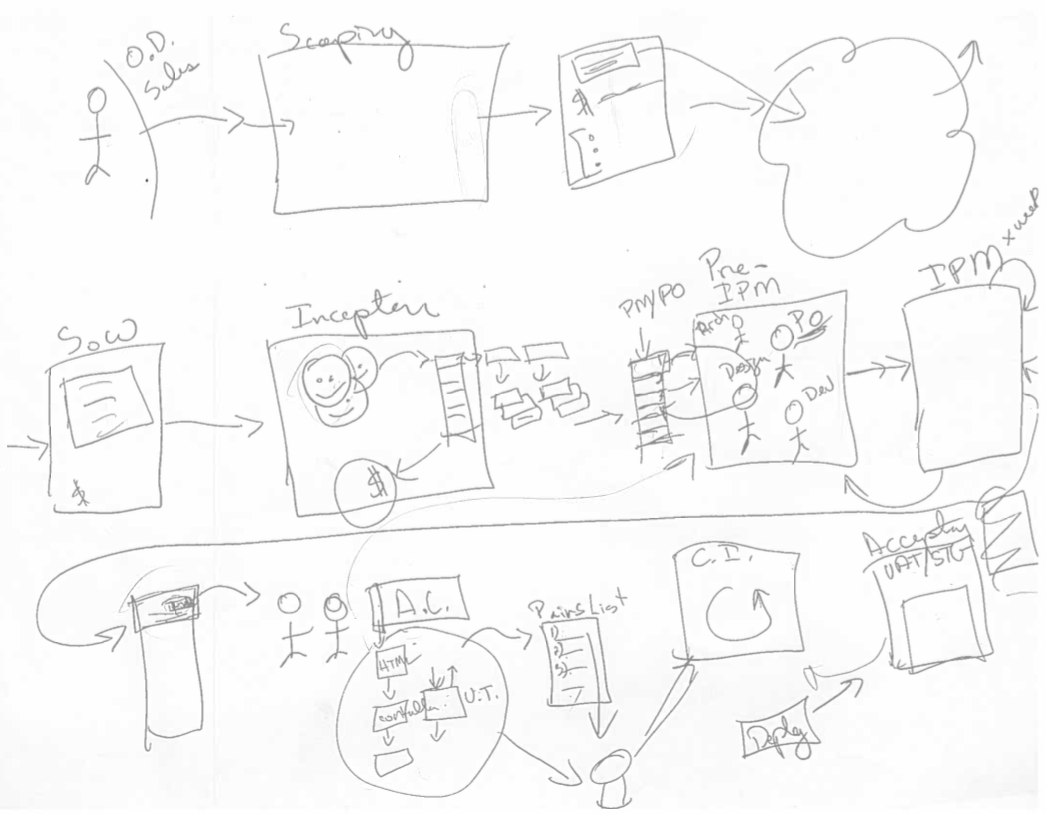
\includegraphics[width=6.5in]{interviews/drawings/2015_08_12_anchor.png}
\caption{\quotes{2015-08-12 Anchor's drawing of software development process}}
\label{2015_08_12_anchor}
\end{figure}

\textbf{Todd:} 	So on a sheet of paper, curious could draw your perspective on our process for software development. 0:00:09

\textbf{Interviewee:}  	Our process for software development.  Where do you want to begin?  Or is that like…  0:00:14

\textbf{Todd:}   Really open.  0:00:15

\textbf{Interviewee:}  	So there's a customer, a potential customer.  And they come and there's some kind of vetting to, at least, get them in the door.  We think that they have interesting idea of some kind, and maybe we ask a couple of questions; so this might be the OD or sales.  Just some minimal vetting and then just enough for them to say: \quotes{you know what, I think we could possibly have a conversation about what it is that you want to have built.}  So then we do a scoping with them, and in that scoping, the input is their general idea.  Usually, it's like pretty vague; It could be from very vague to they totally know what they're talking about both on their problem space and with the solution to look like.  So then the output of that is a document that basically tells them this is what it likely is, and this is how much it's gonna cost, roughly speaking, and these are gonna be the roles and responsibilities, this is what you would be buying.  What just really actually, some amount of hours of some amount of people, different skill, that's what we're actually promising and we'll aim for this thing, but we'll always constantly trying to give you the best value thing as we go along.  So that's some kind of proposal, I don't know exactly what we call that, but it is all part of the scoping.  0:02:00

\textbf{Interviewee:}   And then, I'm gonna draw, like, maybe a number of stops here; by the time I see it, somebody signed, like, an SOW or similar that was possibly, like, but influenced by that scoping value but who knows what negotiations or whatever happened after that; and probably informed by that document, like, what we say we're aiming to deliver.  But this is, I think, this is more like a legal document or as the SOW is more like a legal document whereas the thing that came out of scoping is more of like a \quotes{come work with us} and some of the other stuff around that.  So then, we go into an all of these assumes it's ok.  I'm talking happy path.  Cool?  0:02:59

\textbf{Todd:}  	Yeah, I'm good.  0:03:00

\textbf{Interviewee:}  	So then we do an inception, and this is where, regardless of what we said over here, we get them to get really clear about who is the person that they're targeting; like, ok so it's about a product market fit, who's the market, what's the product gonna be.  So here's this person or persons or personas, and then for each of one those, like, what are the kinds of things that they need to get done, right?  So they've got things that need to happen, that ultimately will result in to some kind of outcomes, and it almost always like it's gonna convert to dollars in some way, shape, or form.  Sometimes it's a non-profit thing and that's slightly different, there's mixed motivation.  So then what we do is we say, \quotes{ok, in order to meet those tasks, what we need is features from the product} and so we're calling out, like, epics, if you will, feature sets, whatever, and then when we start breaking those down into individual stories and these are just sketches at this point.  We're not gonna get all into acceptance criteria right away, it's just like trying to enumerate coz really the outcome of the inception is a backlog. 0:04:43

\textbf{Interviewee:} So you've got some product owner, who culls the outcome of that into a prioritized list of stories, each one of those describes at tiny interaction between this person and the software that we're building.  Ideally, there's variations on that but then, so that's what an individual user story is.  0:04:58

\textbf{Interviewee:}   And then we go to kick off.  So then, we have our first iteration planning meeting where we take as input the prioritized backlog and for each story we go through them.  And by then, the product owner has got them into a point where I call it readied, they've met the definition of ready, which is they have clear acceptance criteria.  There might even be, a pre-IPM where that work is done, as well as, so this is the input is the backlog and the output is the backlog in the pre-IPM.  There are two things that happen, one is that we get clarity early on what the requirement is, and the other is that we get technical input to help with that prioritization and viability, like, ‘ok this may seem simple, like on the face of it', but actually, there's a whole of things that has to happen to make that work, etc. So we surface some of that, the pre-IPM includes somebody from the product side of the house and someone from development, so product owner, development.  Sometimes depending on those, the story can get more complicated, the more requirements, with the greater the variety or the more exotic the product is.  So you might even need someone in from design who is kind of help guiding how this should unfold and the interactions between things because there's all kinds of decisions from that end.  I Imagine, although, we haven't done this yet, in an enterprise client that you might even have somebody from like architecture there, business architecture.  The point of this conversation is to get all of the perspectives that need to be folded into the prioritization and the validation of, that the stories are legit.  0:07:11

\textbf{Todd:}  	Yes.  0:07:12

\textbf{Interviewee:}  	So then that goes into IPM, and this is a straight-forward roll through - the from top to bottom - the backlog, and we go over each story.  We read out title, we read through the acceptance criteria and then the team points each of the stories, the purpose of that is to surface complexity and to get a general, like, understanding, like, common understanding of what this thing actually is, what it is, what's gonna be involved to building it.  0:07:52

\textbf{Todd:}  	Yes.  0:07:53

\textbf{Interviewee:}   	We don't give in to like, we try not to give in to implementation details.  Sometimes, we have to dip down for a second to like verify that we're all speaking the same language, that we're all really envisioning the same kind of thing.  But that usually is surfaced by like, \quotes{I pointed at one and you pointed at five,} and then I would like \quotes{what?}  So then that hopefully prompts a conversation.  If we all said three, it's good enough for now we move on, if we all think it's about the same thing and the product owner doesn't lose their mind hearing that number, then we're all kind of okay.  Then the output of the IPM is individual points on the stories, and we typically go for some amount of horizon so the minimum that I feel comfortable walking out with is at least for the week, so we don't have to, like, break the flow of getting work done before the next IPM because we're gonna do this once a week, these IPMs we're gonna do this once every week. But ideally, a little bit more runway so that we mitigate against that the team haven't jumped out of the flow and also to, like, help the product owner have some room to sort of steer.  If they only have so many points in the stories, then they have to kind of pay the price of reprioritizing. So that's IPM.  Haven't have written a line of code yet.   So then, after IPM, we get working. So out of the backlog, a pair picks up a story and so then that pair looks at the story...  How deep do you want me to go, because I can go all the way down to like testing and stuff.  0:09:48

\textbf{Todd:}  	Sure.  0:09:49

\textbf{Interviewee:}	Ok.  0:09:50

\textbf{Todd:}	This is your diagram.  There's no wrong answer.  0:09:54

\textbf{Interviewee:}  	Alright. Ok.  So, the pair looks at the acceptance criteria and they say, \quotes{hmmm.... what test do I need to write that will help?  Or a set of test that will help if those tests ran green?  I feel really confident that we've met the spirit of that story.}  So they start there.  Usually at pivotal will do typically outside in so that means if we write something that looks like an acceptance test, something that describes very closely what this person with the persona experiences both in what they do, and what they see back from the software.  So we write the starts, we start with a very low fidelity version of that. It's not gonna describe the whole interaction, it might describe the smallest piece of we could possibly articulate; so we start there.  And then we run that test and it fails.  Then we say, \quotes{hmmm, ok, so we're in this architecture, what's the next part that we need to build in order to begin to meet those needs?}  And we work our way down the architecture.  In a typical web app, there's something that's displaying, an HTML page, and then there's something that is probably orchestrating the generation of that HTML, like a controller and usually we try and separate our concerns. We think about these things as we work our way down driven by trying to meet just this one acceptance test.  0:11:26

\textbf{Interviewee:} So along the way what we do is we write individual unit test for the components that have interesting behavior.  The controller does have interesting behavior.  It takes in some input and it makes some decision about what should be the output, what should be the resulting HTML.  And that controller also interacts with other collaborators.  So we have tests that say, are you properly handing off these parameters?  So these really fine-grain unit tests. But the key is that these things are, each time we write these tests, we're setting an expectation on that little tiny piece of the system, in the same way that our acceptance criteria are setting an expectation on the software, and our user stories are setting expectations on the feature .  So forth, all the way back up. We're trying to be needs-based  all the way down as we do this; that's probably good enough.  The details of how that happens varies wildly and even like within this, there are different schools of thought about how that happens.  There's people who believe in writing units for every little thing and people who say \quotes{no, you can set certain bullwarks} and write tests around the bullwarks.  Let everything sort of float in between.  0:12:43